\section{Implementation Part}
\phantomsection
In the previous chapters were discussed the concepts covered by OpenMedia project. The research of the ideas is crucial given that the applications aims a niche which is relatively new in the market, in Moldova it is not even present. To be sure that the platform development start from the right foot, a thorough architecture design, modeled in UML language, was provided in the previous chapter. What follows now is the description of the implementation part. An exhaustive description of every step will be given, including code snippets, which technologies are used and the reason of their choice.

It ought be mentioned that the whole project is mostly written in dynamic language Ruby. Which is why the libraries and frameworks used by OpenMedia are from Ruby world. The secondary language is JavaScript. It is used for building the user interface and for some back end development mostly related to data preprocessing.

\subsection{Obtaining data}
Getting the raw data is the first part in the project cycle. The sources for extracting data are the public channels of media providers from Republic of Moldova. More specific these are Unimedia and Timpul. In further development more sources will be integrated in the system. Extracting each available article is not straightforward task. There are at least two approaches for solving this problem. First one involves social interaction, by contacting media representatives and asking access to the data they dispose of. The second way is to extract the data from the web sites hosted by media providers. Of course the second way is more tricky but at least it avoids the hassle with human interaction and also gives the opportunity to engineer the solution from a developer perspective.

In order to be able to get the data from the web sites one thing ought be clear. Every available article has a unique URL. Once there is a way to get the URL then getting the information is not a problem anymore. The classic way of collecting the URLs from a web page is to launch a crawler. Of course the web spider needs to be trained under the site specifications. This approach is usually chosen by the search engine. Their goal is to extract all the possible content and index the relevant data. The thing is that OpenMedia targets only the pages where only the articles are present. Given that articles from a single source has a unique template not prone to changes, the assumption that the URL also follows a specific pattern might prove useful. After some time and research it was observed that both Unimedia and Timpul article URLs have a similar pattern. Beyond that, in both cases were found unique identifiers in form of a number, for example an article from Unimedia looks like this \emph{http://unimedia.info/stiri/-94630.html}. The natural assumption is that in order to get the URLs for the remaining articles the only thing needed is to decrement the number in the URL string mentioned above. For Timpul media source the process is analogically. One important thing is to know the id range which articles can have. For solving this problem the identifier for the most recent article is extracted from URL. Once this information is available all the articles can be accessed in a simple and iterative manner. And no need for web spiders frameworks are required anymore.

Now that the logical flow of extracting article URLs is present, there are also other requirements like getting the page, saving it to file storage, archiving it first in order to diminish the content size. Also the manner of extracting the articles differ from one source to another. Which means that a custom script should be designed for every particular media source. Nevertheless it is a smart engineering decision to unite the scripts under the same interface. In the following snippet, listing \ref{unimedia_fetchre}, is represented the class used for extracting all articles from Unimedia source. It is an autonomous class with idempotent properties. Every time it runs it checks what is the latest article identifier, what is the most recently saved article and only after that it fetches the missing articles. For extracting web page content the application relies on rest client library \cite{rest_client_ruby}. This library is used in two cases. The first one is for extracting the latest article identifier and the second use case is for fetching article pages themselves. The fact that fetching data is a simple console application does not mean that it shouldn't have a user interface. In order inform the user about the fetching state, a console interface progress bar is used. It provides useful information like how many articles have been fetched, how many remains, what is the estimated time of processing. An example is given in figure \ref{fetcher_progress_bar}.

\begin{figure}[!ht]
\centering
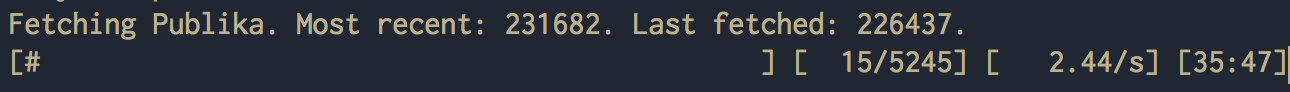
\includegraphics[width=18cm]{3_fetcher_progress_bar}
\caption{Fetcher progress bar}\label{fetcher_progress_bar}
\end{figure}

After fetching the article it is archived and saved to file storage. The handy part of the current implementation is how easy is to integrate one more media source. The only thing needed is implementing a custom fetcher class that will follow the same protocols as FetcherPublica and will have implemented the "run" method. Another required change will be to add on more line of code in the script which controls the fetching process, listing \ref{fetcher_script}. Decoupling the logic offers an increased simplicity when a change in project is required. Following the good practices always generate a good result especially when a project evolves in a changing environment.

\lstinputlisting[language=Ruby, caption={Unimedia fetcher}, label=unimedia_fetchre]{../src/unimedia_fetcher.rb}

\lstinputlisting[language=Ruby, caption={Fetcher script}, label=fetcher_script]{../src/fetcher_script.rb}

Another thing is should be considered is the time of execution. The program heavily relies on network connection given that all the data are available on web. It is also important not to abuse the media sources. In case of too many connections the web server can just block the IP which would lead to an unpleasant situation. The point is that it is not worth to make the script work fast. More than that, in case IP blocking it might even require micro-sleeps between the requests. With this in mind, the resource fetching logic was encapsulated in a separate class. The SmartFetcher class is clever enough to add sleeps before making a request in case that the web server does not respond appropriately. Also it outputs different notification messages in case of unsuccessful request. The good thing is that any fetcher class is encouraged to use the SmartFetcher therefore all the heavy lifting is shifted to an already working part of application. Here is a snippet how the smart fetcher handle errors, listing \ref{smart_fetcher}

\lstinputlisting[language=Ruby, caption={SmartFetcher handling errors}, label=smart_fetcher]{../src/smart_fetcher.rb}

After running the scripts the following was obtained:
\begin{center}
 \begin{tabular}{|c c c |}
 \hline
 Source & Execution time & Storage size \\ [0.5ex] 
 \hline
 Unimedia & 75h & 1.64 GB \\
 \hline
 Timpul & 53h & 1.71 GB \\
 \hline
\end{tabular}
\end{center}

\subsection{Storing data}
Correctly storing data and choosing the right database engine is a tough decision. The problem grows even bigger given the various number of choices available on the market. That is why a lot of factors should be consider. How data would look like. Will it have a lot of relations. What is the estimate number of requests per a period of time. Will it scale in case of a spike of requests. How crucial is to keep the data consistent. Will the business logic imply a lot of updates upon the data. Will data follow a certain schema. What kind of operations are usually applied to data. These are one of the few questions which influence the decision of the database selection.

For OpenMedia project MongoDB was chosen \cite{mongodb}. It is a cross-platform document-oriented database. Being labeled as a NoSQL database it exchanges the traditional table-based relations over JSON type documents with flexible structure. Due to this features it makes the data integration easy and fast in some specific use cases of an application. It makes embedded data very easy to manage. Also it doesn't leave back all the features offered by a traditional RDBMS. It has indexes which work as well as in relational databases. The indexing is happening at embedded field level..

The main reason for choosing this engine is because it is schema-less. Even though the final client part of the application will have a defined schema. MongoDB leverages the flexibility that it provides. Due to the fact that the platform is expected to change its structure and functionality it would be much easier to do so when data is managed by MongoDB. Another critical part is data preprocessing. The number of phases in which data might shape is hard to forecast. The entire system behaves very much like a live organism. In order to easily grasp and adapt under the new requirements MongoDB will offer means for easily prototyping the needed result.

Another important tool offered by MongoDB is the support for native MapReduce operations. OpenMedia relies heavily on this type of operations. MapReduce is fundamental in the data preprocessing part. There is no doubt that this part could be managed at the application level, but it makes more sens to use the tools which offers easy and elegant solutions to the problem.

The second step of the application is to extract the articles content from the HTML files stored on disk space and save to a database, more accurately to MongoDB. This results in writing a set of XML parsers which will be executed on the fetched data. The parsers should be adapted under the custom preferences of a specific media channel. As only two sources are targeted by OpenMedia results in two custom classes. The implementation concept is analogically the same as the fetching part of the system. A set of classes that follow the same protocol such that they can be easily managed. In listing \ref{timpul_parser} is represented the implementation of the most relevant methods of TimpulParsert class.

\lstinputlisting[language=Ruby, caption={TimpulParser parse and save methods}, label=timpul_parser]{../src/timpul_parser.rb}

The code represents the idea how a parser works. Nokogiri library was used for solving the specific problem of HTML parsing \cite{nokogiri_gem}. It is a easy to use library which is able to digest an XML input and return a set of nodes in form of ruby objects with enhanced functionality. In the end the consisted data is extracted in form of a plain Ruby hash and saved to database. Now the important part comes, the communication between the Ruby language and MongoDB. Naturally a ruby library is used for achieving the communication. In context of OpenMedia is specifically used Mongoid gem \cite{mongoid_gem}. An ORM is an API written in a specific language which offers a communication between a database and a programming language. It does more than that, it has the purpose to map the fields from a database to an class instance understood by the programming language. Thus making data accessing activity in a manner easily understood by the OOP language. A well implemented ORM comes hand in hand with a rich and powerful DSL. Of course not all the feature could be accessed through an intermediary DSL but at least it provides the most common operations. On the other hand when it comes to MongoDB, the native API is accessible in JavaScript. Which means that is realistic to create an ORM almost as powerful as the native API. Mongoid is a library which fulfills the necessity of the OpenMedia platform. It even allows injecting JavaScript code. In order to be able to operate with the database using Mongoid a set of classes, usually called models, needs to be define which comply a certain protocol. The class should included the Mongoid::Document interface and all the fields should be specified alongside with their type. An example of such a class is provided in the following listing \ref{mongoid_model}.

\lstinputlisting[language=Ruby, caption={ParsedPage Mongoid model}, label=mongoid_model]{../src/mongoid_model.rb}


\subsection{NLP processing}
The natural language processing is one of the most challenging part of the project. And there are few reasons which are backing up the problem. The major problem is that the data used in OpenMedia project is just text in Romanian language. There is nothing wrong with Romanian. The problem lies in the libraries available for use. In order to successfully implement a decent NLP library it requires a lot of tedious work. And it can only be done within a joint collaboration between a group of computer science engineers and experts in the specific language. A modern NLP library is built using probabilistic models and machine learning that requires a lot of data under a special format. The special format should be provided under the form of big chunks of text manually annotated with metadata such as the part of speech, what is the text token etc. The point is that creating such a library is a laborious process that usually involves specially trained stuff with a PhD degrees. Overall there are already available frameworks which does successfully does the text processing part. The tricky thing is that most of them are for English language. When it comes to Romanian the sources are very limited.

Luckily there are few universities from Romania which does research in this area and already have successfully implemented a set of libraries that can be used in context of OpenMedia. Currently there are two sources which are able to provide such a service. Both are doing so only in form of a online service over SOAP protocol. The first source is Universitatea "Alexandru Ioan Cuza" din Iași\cite{uaic}. The second source is Institutul de Cercetări pentru Inteligență Artificială "Mihai Drăgănescu", Academia Română\cite{racai}. In scope of the currently project was chosen the least source only because it was first found. No benchmarks were done over the sources, but as a future perspective there will be done a set of tests which will check which source is more reasonable to use. Or if it is possible to use both sources at the same time. Given that NLP is a costly and a long process it would be fair to divide the labor. It is rather unfortunate that neither sources does not provide the service under a form of library. There are more issues when it comes to using a SOAP service. The first one is latency, every service provided on the web is much slower in comparison to natively running a software. The second problem is the dependency. When an entire product relies on an external service, the entire infrastructure is very fragile. What if at some point in time the service will simply shutdown will this mean the end of product? And the last issue is the ethical part. To build a product that could possibly be sold on the market on top of sources provided by an university is not the correct business approach.

Coming back to the implementation part. The NLP operations were encapsulated in a separate class, RacaiBuilder. The operations represent nothing more but SOAP calls to one of the mentioned services. Under the class hood there's nothing more than an adapter to a external web services. For a successful implementation "savon" library was used \cite{savon_gem}. It is a ruby gem which encapsulates the hassle of operating with SOAP protocol by providing a simple and well documented API. THe class RacaiFetcher was constructed in form of a builder in order to give the developer the freedom to chose the order of operations. In the following  listing \ref{racai_builder} is represented some of the NLP methods and the client SOAP client management withing savon gem.

\lstinputlisting[language=Ruby, caption={ParsedPage Mongoid model}, label=racai_builder]{../src/racai_builder.rb}

So far so good. Now that there is class which is able to apply NLP actions upon an input is a great achievement in the project. What remains is to extract the parsed articles from MongoDB and run them through NLP class. Also the structure of the output result will be stored back into MongoDB under a different format. Most of the queries will be done by a specific word. Which suggests that it would be a better idea to store every word as a separate record. Of course every record will also contain additional metadata which will permit to extract the needed result for data visualization. As it was mentioned, using web service for a big amount of data takes a big amount of time. Parsing the and extracting articles to MongoDB resulted in 453 Mb of textual data. It is not a big amount overall, but from analysis perspective it will still require a long period of time to execute NLP operations, especially when used via a SOAP service. In the end the execution time on an average home PC took around 14 days. And it generated 9.2 GB of data.

\subsection{Preparing data for visualization}
The NLP operations were executed on the raw textual data. This brought data one step closer to the visualization part. To be more clear it only needs to undergo the data preprocessing phase in order to be ready for data visualization. Of course there was an initial attempt to skip this phase of the cycle. By having at disposal mapreduce tool offered by mongodb it was easy to prototype how user requests would look like under a format of a mapreduce. In listing \ref{long_map_reduce} is represented the source code of such a task.

\lstinputlisting[language=Java, caption={User mapreduce request on unprocessed data}, label=long_map_reduce]{../src/long_map_reduce.js}

The execution time of the code shown above on an average PC takes around 5 minutes. The result is understandable considering that the dataset is around 10 GB. Still, it is a very long time for a single user request. The immediate feedback is crucial feature within a client based application. The bottleneck proves to be the large dataset. This means that data should go through a compression process but at the same time remain consistent. The NLP step generated a dataset in a format of every word in every article with metadata such as article\_id, published time, part of speech and the source. What user requires is the number of mentions per month and the media source of a specified word. In order to meet the user requirements the data can be stored in form of  {word, mentions, year, month, source}. In listing \ref{bend_map_reduce} is represented a mapreduce task which bends the data under the user requirements.

\lstinputlisting[language=Java, caption={Mapreduce job for data compression}, label=bend_map_reduce]{../src/bend_map_reduce.js}

It looks quite similar to the previous mapreduce. The only different thing is that it runs once there are data updates but not at every user requests. The resulted data size is 456 MB. This is a number that can be worked with. More than that, it has such a structure that the user requests no longer need to execute mapreduce tasks. It is just a simple query with a simple conditional which takes around 0.5 seconds. As it was mentioned before that MongoDB offers indexing features. After composing and index by the word field the query result improved even better. It got to immediate responses around few milliseconds. Data preprocessing is indeed an astonishing improvement to the system. It decreased the request time from five minutes to few milliseconds. Alongside the data compression mapreduce job another compression task is required. The job is intended to computes the number of published articles for every month for every media channel. This data is used to compute the a specific ratio. The number of articles which have the mentioned the word over the number of published articles in a single month.

\subsection{Visualizing the data}
Data visualization is the part that matters to the end user. Everything done until now does not have a value if data is not represented under a human readable format. It is important that data should be represented in such way that it would communicate a message. A message that is clear enough and from which viable conclusions can be drawn. In context of OpenMedia the only method for displaying data is the line chart. For every user requests there are available only two line charts. Even though it might be not very much, building the whole infrastructure took a lot of time and research. Besides in case there is a sudden idea to add a new type of search, or a new type of data visualization the implementation phase would be very easy due to the fact that there is a platform which backs up and does a lot of hard work regarding data flow.

The data visualization happens in a browser page. This concludes that the tools for building plots are JavaScrpit based libraries. OpenMedia platform uses D3 library for constructing visual data representations \cite{d3}. D3, coming from Data-Driven Documents, is a library used for constructing dynamic and interactive data visualization in a web browser. It heavily relies on SVG, HTML5 and CSS standards. The most powerful point of this library is that it gives a great control over the final result. Embedded within an HTML webpage, the JavaScript D3.js library uses pre-built JavaScript functions to select elements, create SVG objects, style them, or add transitions, dynamic effects or tooltips to them. These objects can also be widely styled using CSS. Large datasets can be easily bound to SVG objects using simple D3.js functions to generate rich text/graphic charts and diagrams. The data can be in various formats, most commonly JSON, comma-separated values (CSV) or geoJSON, but, if required, JavaScript functions can be written to read other data formats.

As it was mentioned there are only two types of line plots for every user requests. The line-plots depicts how in how many articles the specified word was mentioned in a month. The first chart computes the word frequency in relation with the total amount of articles published by the source in that month. The second plot simply shows the number of mentions of the word. In order to browse the plot information in a easy manner it was enhanced with tooltip feature. When a plot is hovered it shows how many mentions are present and what is the date to which the the data relates. A representation of the result can be observed in figure \ref{frequency_plot} and figure \ref{mentions_plot}.

\begin{figure}[!ht]
\centering
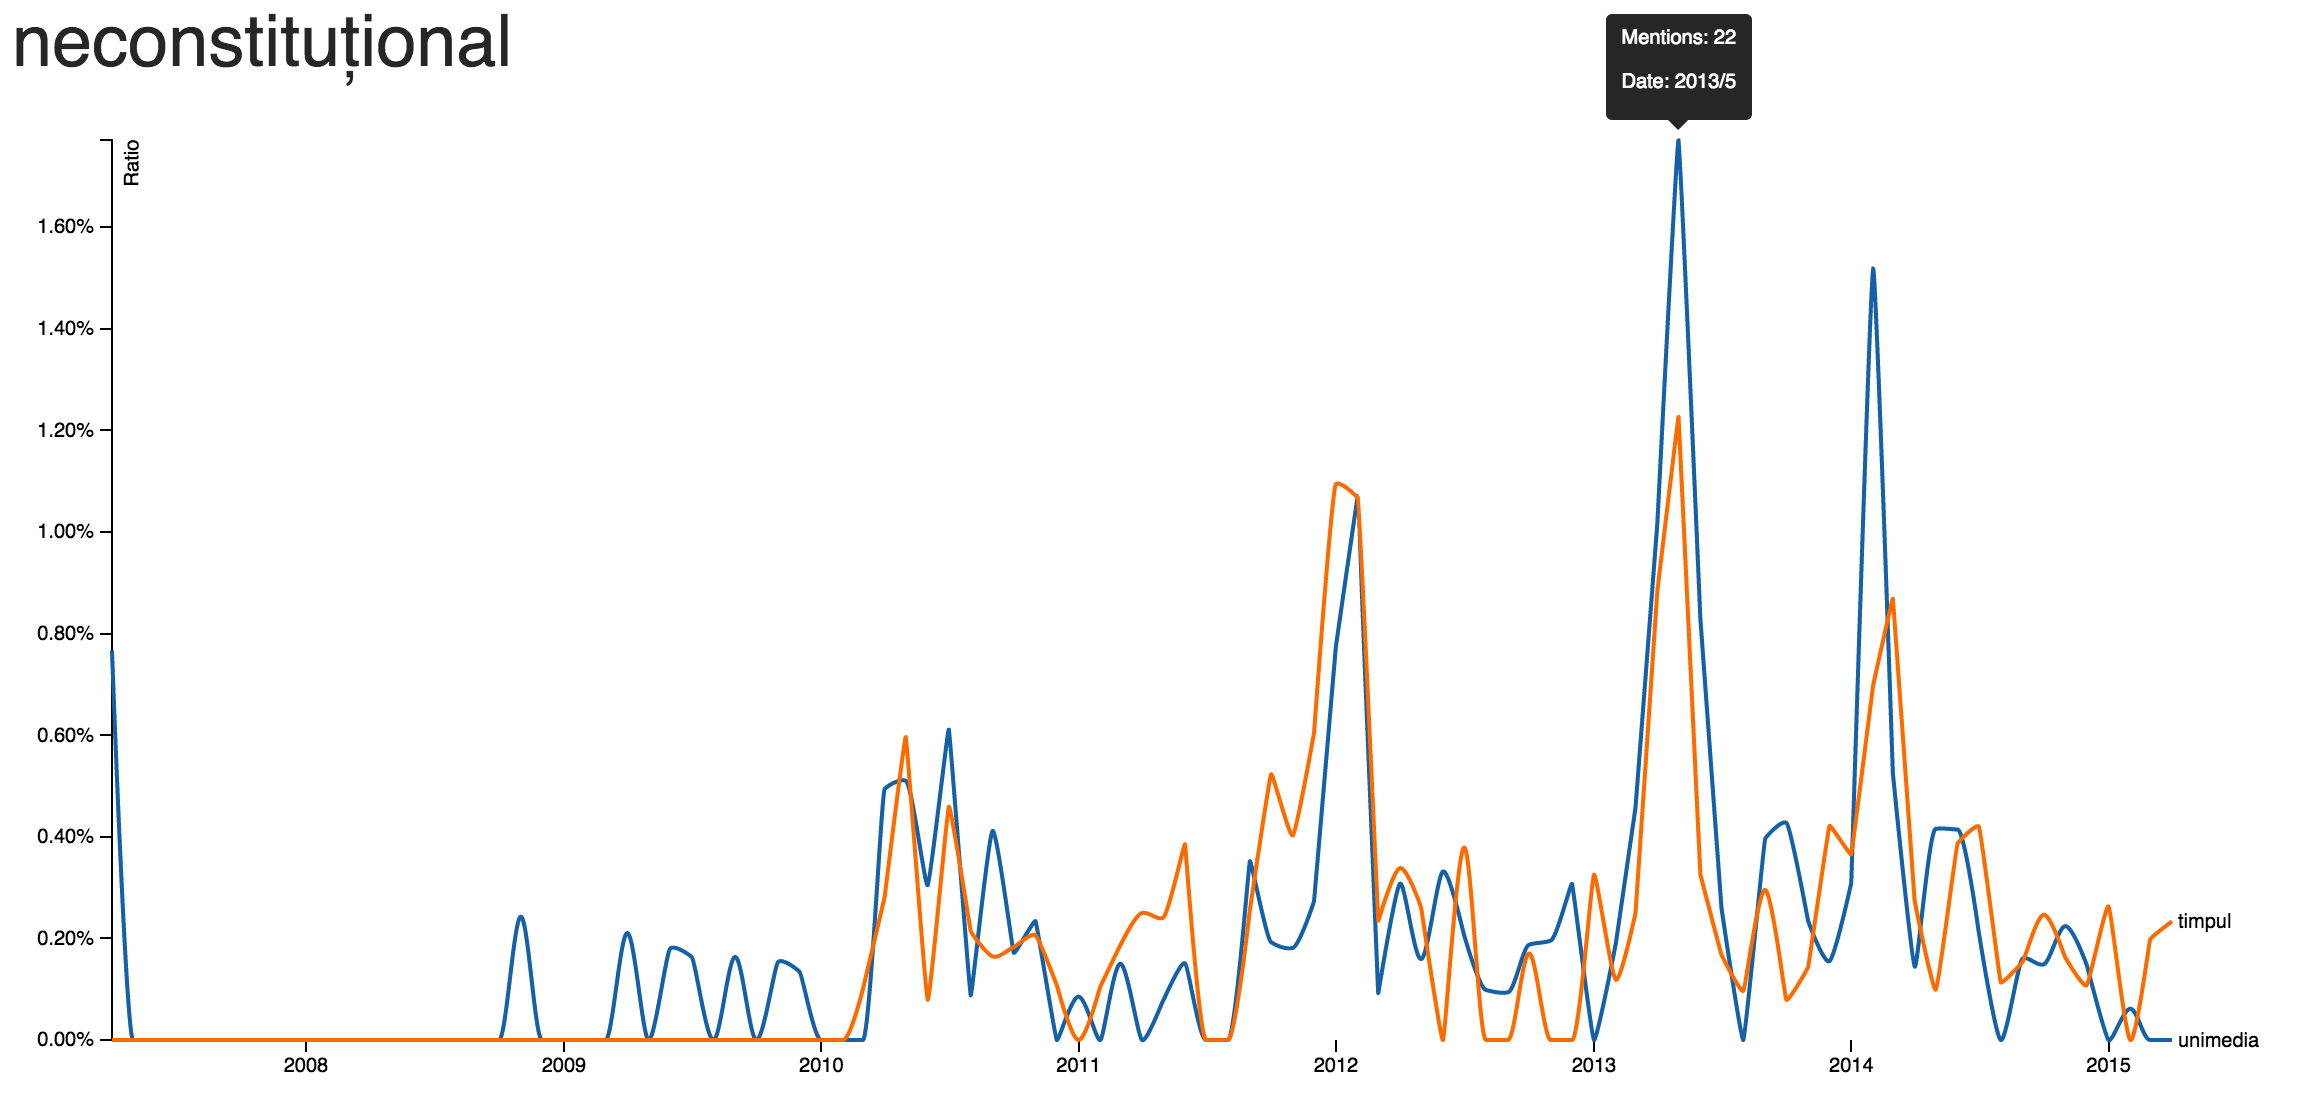
\includegraphics[width=15cm]{3_frequency_plot}
\caption{Frequency line plot}\label{frequency_plot}
\end{figure}

\begin{figure}[!ht]
\centering
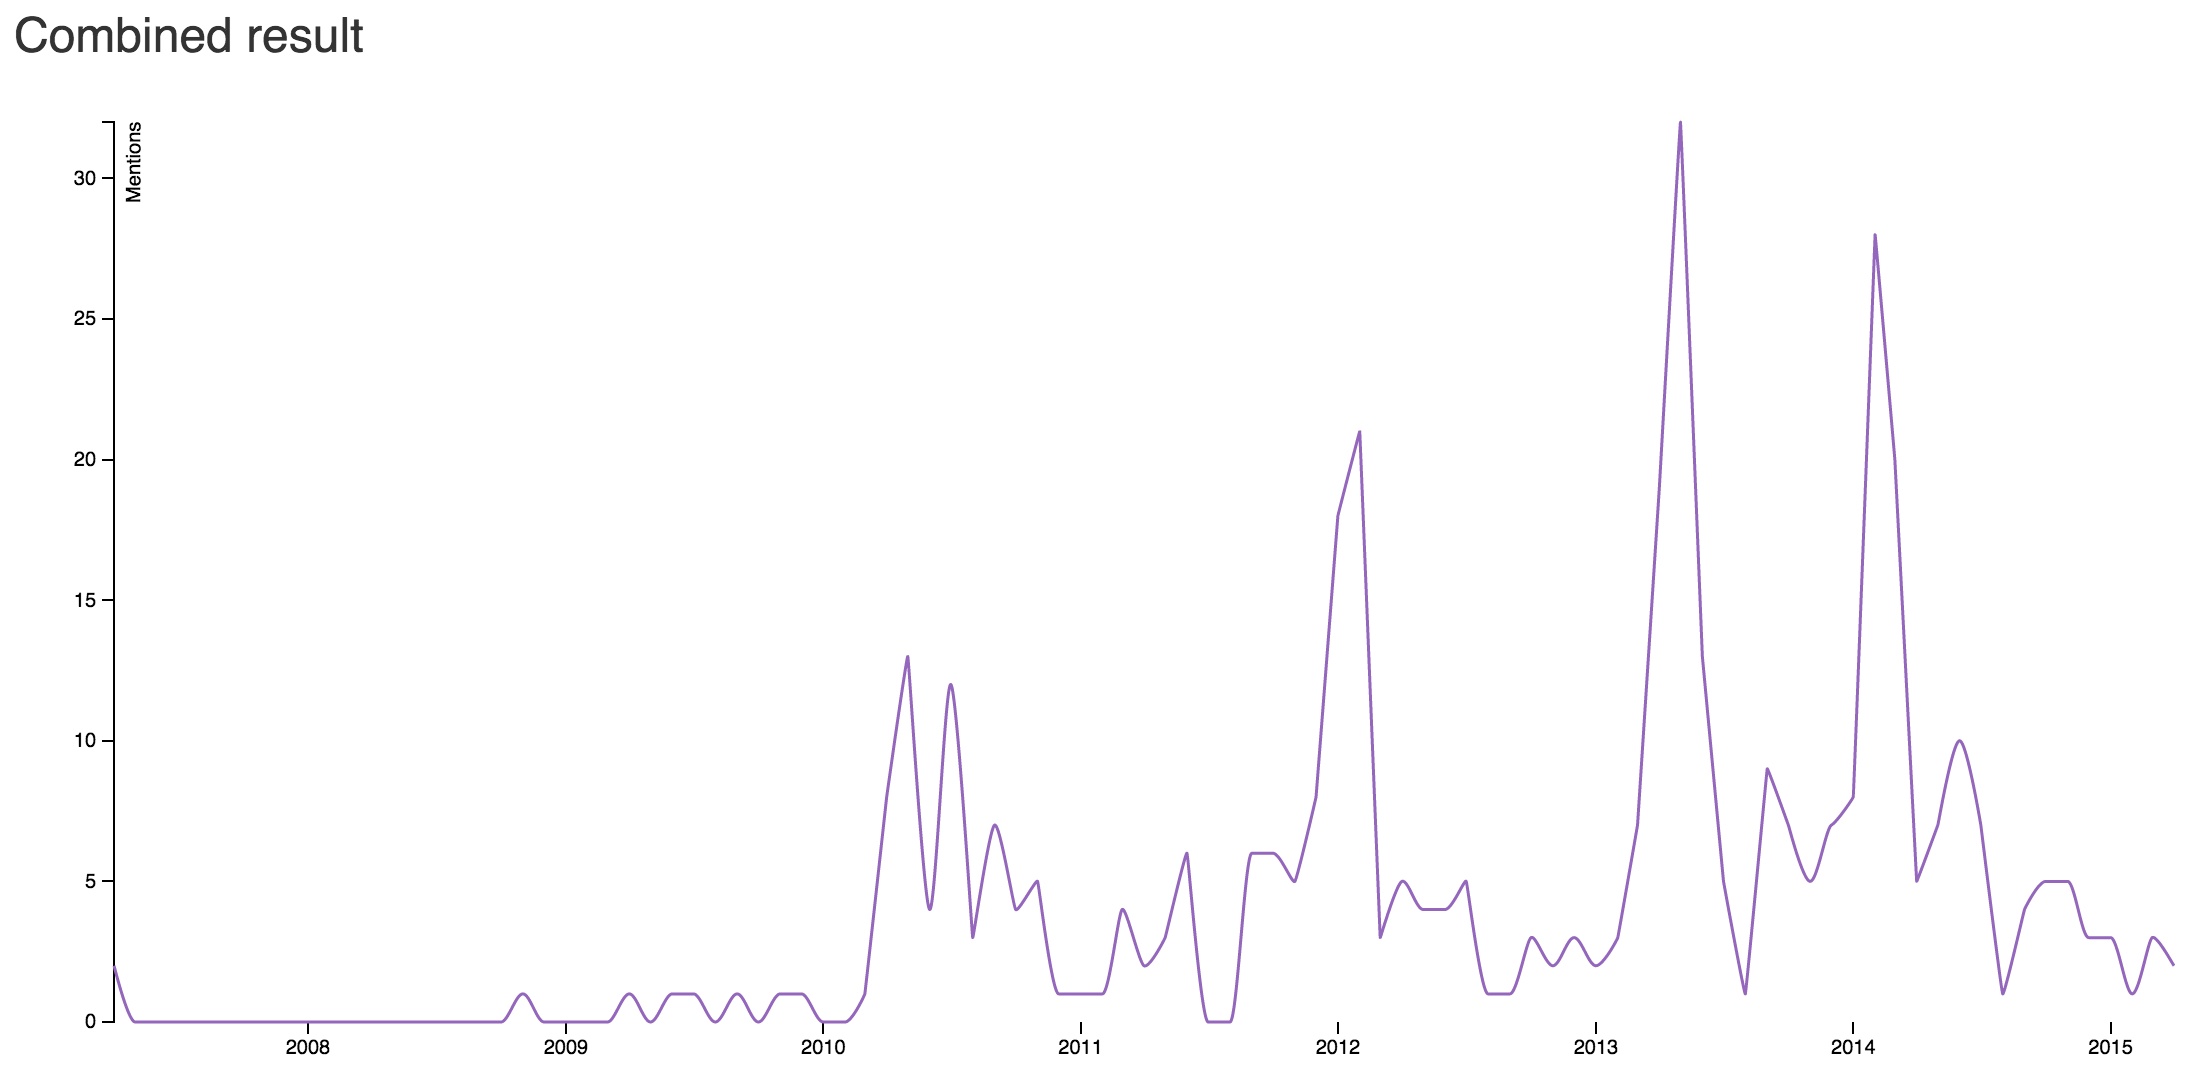
\includegraphics[width=15cm]{3_mentions_plot}
\caption{Mentions line plot}\label{mentions_plot}
\end{figure}

\subsection{Providing the UI}
To provide a good user interface is crucial to any software engineer. The whole point of creating an application is not how it works in the background, on how many clusters it runs on, or how efficiently the data is stored. All this details does not matter as long as a good user interface is present. More than that all the mentioned details combined can help to create the great user experience. Making a good application is not about creating a bunch of functionalities. It is about designing a flow of actions that feels natural to those who end up using the product.

OpenMedia platform uses browser web page application for the client side. A web platform usually relies on HTTP protocol concluding that in order to start the product a tool for building web applications is required. The chosen technology is Sinatra\cite{sinatra}. Sinatra is a ruby based framework. It is very simple to use and is perfect for building small applications. In listing \ref{sinatra_app} is represented a snipped of code which proves how simple is to implement the business logic of a specific HTTP method on a given URL. The given code is almost everything needed for running the applications. The hassles starts when trying add different components to the application. Due to the fact the Sinatra is very simple it requires a bit of tunning when it comes adding modules.

\lstinputlisting[language=Ruby, caption={HTTP requests handling implemented with Sinatra}, label=sinatra_app]{../src/sinatra_app.rb}

The client part of the application was initially design having in mind that user requests will launch time-consuming tasks. In order to run the jobs in the background and keep the UI interactive, Sidekiq technology was used\cite{sidekiq}. It is ruby library used for launching asynchronous tasks. For dealing with long requests, simple threads could be used but this would mean loading the applications server. The good thing about Sidekiq is that it can run on a separate server. Another thing is that it based on message queue system. Thus the amount of workers running simultaneously can be easily managed. Sidekiq uses Redis database for queuing jobs. Redis is a key-value database\cite{redis} that is often chosen for solving different type of solutions which involves volatile data. The most common use is data caching. Due to the fact that the data is stored in RAM it offers a very fast IO operations. Besides it supports a various built in operations. In listing \ref{sidekiq_worker} is represented a worker class used in OpenMedia.

\lstinputlisting[language=Ruby, caption={Sidekiq worker class}, label=sidekiq_worker]{../src/sidekiq_worker.rb}

Now that the time resourceful task execution is separated to an another node, a new problem surfaces. How to notify the user that a specific task has finished. The browser web page and a Sidekiq worker are two totally decoupled instances. In oder to solve this issue an additional node is added to the platform which does the communication between theses two sides. Faye tool is used for this part of the application \cite{faye}. It is a publisher subscriber system which relies on web sockets. When a request submits a search request Sinatra responds immediately with a specific token, it also launches a task on Sidekiq. What happens on the client browser is that after the token was received, it subscribes to a Faye channel specified by the token string. The worker is also aware of the token. After finishing the job it sends an HTTP requests to the channel. The client receives a messages thus a notification is rendered. In figure \ref{notifications} is illustrated an example.

\begin{figure}[!ht]
\centering
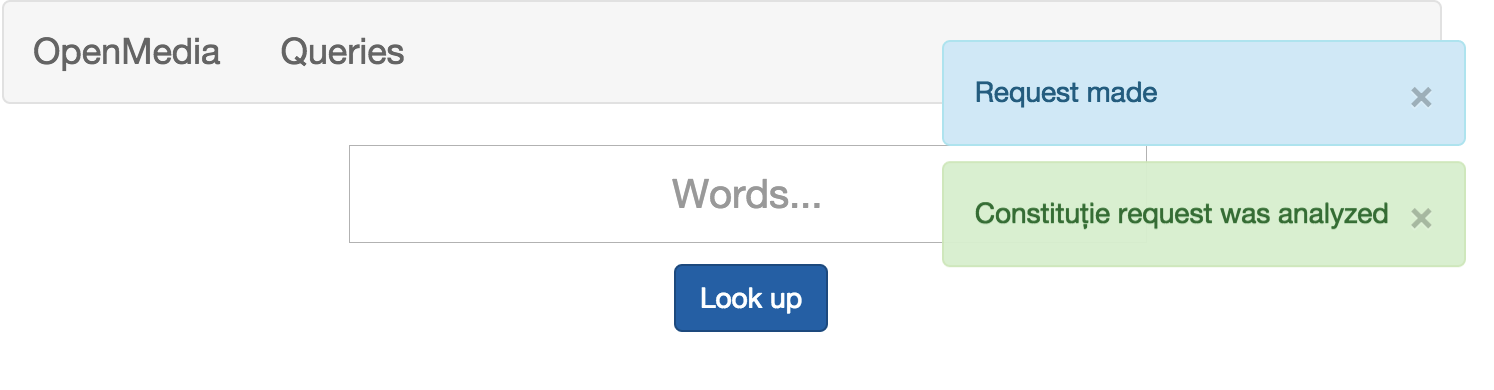
\includegraphics[width=15cm]{3_notifications}
\caption{An example of notification}\label{notifications}
\end{figure}


\clearpage